% Options for packages loaded elsewhere
% Options for packages loaded elsewhere
\PassOptionsToPackage{unicode}{hyperref}
\PassOptionsToPackage{hyphens}{url}
%
\documentclass[
  ignorenonframetext,
]{beamer}
\newif\ifbibliography
\usepackage{pgfpages}
\setbeamertemplate{caption}[numbered]
\setbeamertemplate{caption label separator}{: }
\setbeamercolor{caption name}{fg=normal text.fg}
\beamertemplatenavigationsymbolsempty
% remove section numbering
\setbeamertemplate{part page}{
  \centering
  \begin{beamercolorbox}[sep=16pt,center]{part title}
    \usebeamerfont{part title}\insertpart\par
  \end{beamercolorbox}
}
\setbeamertemplate{section page}{
  \centering
  \begin{beamercolorbox}[sep=12pt,center]{section title}
    \usebeamerfont{section title}\insertsection\par
  \end{beamercolorbox}
}
\setbeamertemplate{subsection page}{
  \centering
  \begin{beamercolorbox}[sep=8pt,center]{subsection title}
    \usebeamerfont{subsection title}\insertsubsection\par
  \end{beamercolorbox}
}
% Prevent slide breaks in the middle of a paragraph
\widowpenalties 1 10000
\raggedbottom
\AtBeginPart{
  \frame{\partpage}
}
\AtBeginSection{
  \ifbibliography
  \else
    \frame{\sectionpage}
  \fi
}
\AtBeginSubsection{
  \frame{\subsectionpage}
}
\usepackage{iftex}
\ifPDFTeX
  \usepackage[T1]{fontenc}
  \usepackage[utf8]{inputenc}
  \usepackage{textcomp} % provide euro and other symbols
\else % if luatex or xetex
  \usepackage{unicode-math} % this also loads fontspec
  \defaultfontfeatures{Scale=MatchLowercase}
  \defaultfontfeatures[\rmfamily]{Ligatures=TeX,Scale=1}
\fi
\usepackage{lmodern}

\usetheme[]{metropolis}
\ifPDFTeX\else
  % xetex/luatex font selection
\fi
% Use upquote if available, for straight quotes in verbatim environments
\IfFileExists{upquote.sty}{\usepackage{upquote}}{}
\IfFileExists{microtype.sty}{% use microtype if available
  \usepackage[]{microtype}
  \UseMicrotypeSet[protrusion]{basicmath} % disable protrusion for tt fonts
}{}
\makeatletter
\@ifundefined{KOMAClassName}{% if non-KOMA class
  \IfFileExists{parskip.sty}{%
    \usepackage{parskip}
  }{% else
    \setlength{\parindent}{0pt}
    \setlength{\parskip}{6pt plus 2pt minus 1pt}}
}{% if KOMA class
  \KOMAoptions{parskip=half}}
\makeatother


\usepackage{longtable,booktabs,array}
\usepackage{calc} % for calculating minipage widths
\usepackage{caption}
% Make caption package work with longtable
\makeatletter
\def\fnum@table{\tablename~\thetable}
\makeatother
\usepackage{graphicx}
\makeatletter
\newsavebox\pandoc@box
\newcommand*\pandocbounded[1]{% scales image to fit in text height/width
  \sbox\pandoc@box{#1}%
  \Gscale@div\@tempa{\textheight}{\dimexpr\ht\pandoc@box+\dp\pandoc@box\relax}%
  \Gscale@div\@tempb{\linewidth}{\wd\pandoc@box}%
  \ifdim\@tempb\p@<\@tempa\p@\let\@tempa\@tempb\fi% select the smaller of both
  \ifdim\@tempa\p@<\p@\scalebox{\@tempa}{\usebox\pandoc@box}%
  \else\usebox{\pandoc@box}%
  \fi%
}
% Set default figure placement to htbp
\def\fps@figure{htbp}
\makeatother





\setlength{\emergencystretch}{3em} % prevent overfull lines

\providecommand{\tightlist}{%
  \setlength{\itemsep}{0pt}\setlength{\parskip}{0pt}}



 


\setbeamerfont{title}{size=\large}
\usepackage{hyperref}
\setbeamertemplate{footline}[frame number]
\usepackage{tikz}
\usetikzlibrary{arrows.meta, positioning, shapes.geometric, fit, backgrounds, calc}
\usepackage{booktabs}
\usepackage{xcolor}
\usepackage{array}
\definecolor{mblue}{RGB}{35,55,100}
\makeatletter
\@ifpackageloaded{caption}{}{\usepackage{caption}}
\AtBeginDocument{%
\ifdefined\contentsname
  \renewcommand*\contentsname{Table of contents}
\else
  \newcommand\contentsname{Table of contents}
\fi
\ifdefined\listfigurename
  \renewcommand*\listfigurename{List of Figures}
\else
  \newcommand\listfigurename{List of Figures}
\fi
\ifdefined\listtablename
  \renewcommand*\listtablename{List of Tables}
\else
  \newcommand\listtablename{List of Tables}
\fi
\ifdefined\figurename
  \renewcommand*\figurename{Figure}
\else
  \newcommand\figurename{Figure}
\fi
\ifdefined\tablename
  \renewcommand*\tablename{Table}
\else
  \newcommand\tablename{Table}
\fi
}
\@ifpackageloaded{float}{}{\usepackage{float}}
\floatstyle{ruled}
\@ifundefined{c@chapter}{\newfloat{codelisting}{h}{lop}}{\newfloat{codelisting}{h}{lop}[chapter]}
\floatname{codelisting}{Listing}
\newcommand*\listoflistings{\listof{codelisting}{List of Listings}}
\makeatother
\makeatletter
\makeatother
\makeatletter
\@ifpackageloaded{caption}{}{\usepackage{caption}}
\@ifpackageloaded{subcaption}{}{\usepackage{subcaption}}
\makeatother

\usepackage{bookmark}
\IfFileExists{xurl.sty}{\usepackage{xurl}}{} % add URL line breaks if available
\urlstyle{same}
\hypersetup{
  pdfauthor={Giorgio Arcara},
  hidelinks,
  pdfcreator={LaTeX via pandoc}}


\author{Giorgio Arcara}
\date{}

\begin{document}


\begin{frame}
\title{Metodologia della Ricerca Clinica\\
\vspace{0.5em}
{\normalsize \textbf{13. Review e Meta-analisi}}}
\author{Giorgio Arcara,\\ Università di Padova \\ IRCCS San Camillo, Venezia}
\titlegraphic{
\vspace*{7cm}
\includegraphics[scale=0.15]{Figures/LogoSanCamilloIRCCS_Unipd_alpha.png}
\hfill \includegraphics[scale=0.15]{Figures/CC_license_3_0.png}
}
\maketitle
\end{frame}

\section{12.1 Sintesi delle evidenze}\label{sintesi-delle-evidenze}

\begin{frame}{Premessa}
\phantomsection\label{premessa}
% [IMMAGINE SUGGERITA: classica piramide EBM a 6 livelli con colori graduali]
\begin{center}
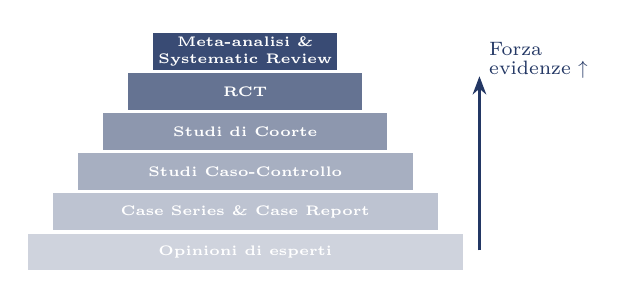
\begin{tikzpicture}[scale=0.85, font=\tiny]
  \foreach \i/\lbl/\shade in {
    0/{Opinioni di esperti}/22,
    1/{Case Series \& Case Report}/30,
    2/{Studi Caso-Controllo}/40,
    3/{Studi di Coorte}/52,
    4/{RCT}/70,
    5/{Meta-analisi \& \\ Systematic Review}/90
  }{
    \pgfmathsetmacro{\w}{6.5 - \i*0.75}
    \pgfmathsetmacro{\y}{\i*0.6}
    \fill[mblue!\shade] (-\w/2, \y) rectangle (\w/2, \y+0.55);
    \node[white, font=\tiny\bfseries, align=center] at (0, \y+0.27) {\lbl};
  }
  \node[right, font=\scriptsize, mblue] at (3.5, 3.3) {Forza};
  \node[right, font=\scriptsize, mblue] at (3.5, 3.0) {evidenze $\uparrow$};
  \draw[-{Stealth}, mblue, thick] (3.5, 0.3) -- (3.5, 2.9);
\end{tikzpicture}
\end{center}
\vspace{-0.3em}
\small La piramide \textbf{Evidence Based Medicine} (EBM) pyramid organizza i disegni per \textbf{forza delle evidenze prodotte}.
\end{frame}

\begin{frame}{Perché sintetizzare le evidenze?}
\phantomsection\label{perchuxe9-sintetizzare-le-evidenze}
\small

Nessuno studio singolo è sufficiente per fondare la pratica clinica:

\begin{itemize}\footnotesize
\item I campioni sono limitati $\Rightarrow$ stime instabili \pause
\item I risultati possono contraddirsi \pause
\item È molto dispendioso leggere tutti gli articoli originali \pause
\item Le linee guida devono basarsi su un corpus di evidenze, non su singoli lavori.
\end{itemize}
\end{frame}

\begin{frame}{A complicare la cose}
\phantomsection\label{a-complicare-la-cose}
\begin{center}
\includegraphics[width=0.2\linewidth,height=\textheight,keepaspectratio]{Figures/triangle.png}
\end{center}

\begin{itemize}
\item
  Anche se un effetto è \textbf{vero} statisticamente non tutti gli
  studi mostreranno quell'effetto \pause
\item
  Anche se un effetto \textbf{non è vero}, statisticamente alcuni studi
  potrebbero mostrare quell'effetto.
\end{itemize}

(c'entra il fatto che lavoriamo su \emph{campioni} estratti da
\emph{popolazioni})
\end{frame}

\begin{frame}{Sintesi delle evidenze}
\phantomsection\label{sintesi-delle-evidenze-1}
Con \textbf{Sintesi delle evidenze} si intende il processo di raccolta,
organizzazione e valutazione complessiva di risultati esistenti su uno
specifico ambito.

\begin{center}
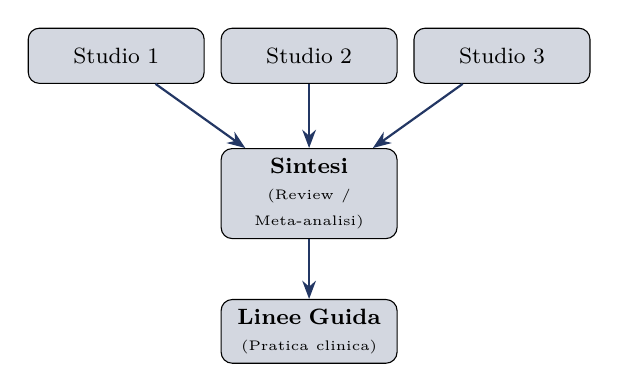
\begin{tikzpicture}[scale=0.7,
                    box/.style={draw,rounded corners,fill=mblue!20,text width=2cm,
                    align=center,font=\footnotesize,minimum height=0.7cm},
                    arr/.style={-{Stealth},mblue,thick}
]
\node[box] (s1) at (-3.5,0) {Studio 1};
\node[box] (s2) at ( 0,0) {Studio 2};
\node[box] (s3) at ( 3.5,0) {Studio 3};
\node[box] (sr) at ( 0,-2.5) {\textbf{Sintesi}\\\tiny (Review / Meta-analisi)};
\node[box] (lg) at ( 0,-5.0) {\textbf{Linee Guida}\\\tiny (Pratica clinica)};
\draw[arr] (s1)--(sr); \draw[arr] (s2)--(sr); \draw[arr] (s3)--(sr);
\draw[arr] (sr)--(lg);
\end{tikzpicture}
\end{center}
\end{frame}

\begin{frame}{Tipi di Review: Panoramica}
\phantomsection\label{tipi-di-review-panoramica}
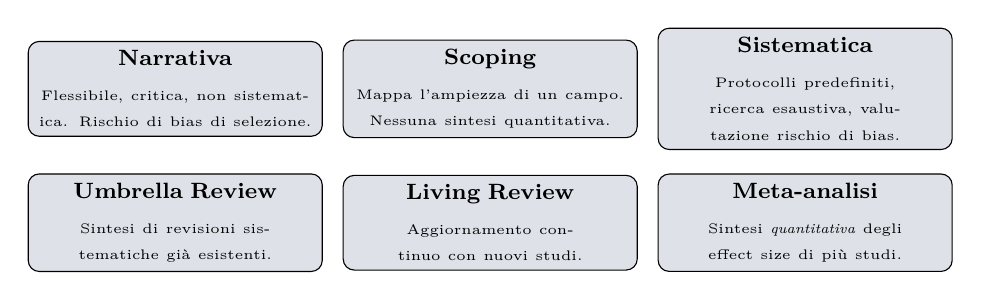
\begin{tikzpicture}[
  box/.style={draw,rounded corners,fill=mblue!15,text width=3.5cm,
  align=center,font=\footnotesize,minimum height=1.2cm},
]
\node[box] at (-5,1.2) {\textbf{Narrativa}\\[3pt]\tiny Flessibile, critica, non sistematica. Rischio di bias di selezione.};
\node[box] at (-1,1.2)    {\textbf{Scoping}\\[3pt]\tiny Mappa l'ampiezza di un campo. Nessuna sintesi quantitativa.};
\node[box] at (3,1.2)  {\textbf{Sistematica}\\[3pt]\tiny Protocolli predefiniti, ricerca esaustiva, valutazione rischio di bias.};
\node[box] at (-5,-0.5){\textbf{Umbrella Review}\\[3pt]\tiny Sintesi di revisioni sistematiche già esistenti.};
\node[box] at (-1,-0.5)   {\textbf{Living Review}\\[3pt]\tiny Aggiornamento continuo con nuovi studi.};
\node[box] at (3,-0.5) {\textbf{Meta-analisi}\\[3pt]\tiny Sintesi \emph{quantitativa} degli effect size di più studi.};
\end{tikzpicture}
\end{frame}

\begin{frame}{Revisione Sistematica}
\phantomsection\label{revisione-sistematica}
\small

\textbf{Obiettivo}: sintetizzare le evidenze su un specifico aspetto di
interesse scientifico.

\textbf{Caratteristiche}:

\begin{itemize}
\item
  Protocollo predefinito e registrato (es.~PROSPERO) \emph{prima} di
  iniziare la ricerca.
\item
  Ricerca esaustiva : più banche dati (PubMed, Embase, PsycINFO,
  Cochrane), letteratura grigia, reference list degli studi inclusi.
\item
  Doppia selezione : due revisori indipendenti selezionano gli studi e
  risolvono i disaccordi per consenso o terzo revisore.
\item
  Valutazione del rischio di bias: per ogni studio incluso (es.~RoB 2
  per RCT, ROBINS-I per studi osservazionali).
\item
  Output può essere narrativo o, se possibile, meta-analisi
  quantitativa.
\end{itemize}

\tiny PROSPERO:
\url{https://www.crd.york.ac.uk/prospero/}\textbackslash{} RoB 2:
\href{https://sites.google.com/site/riskofbiastool/welcome/rob-2-0-tool?authuser=0}{\underline{ROB2 link}}
\end{frame}

\begin{frame}{Review sistematica: vantaggi e svantaggi}
\phantomsection\label{review-sistematica-vantaggi-e-svantaggi}
\textbf{vantaggi}:

\begin{itemize}
\tightlist
\item
  meno soggetta a bias
\item
  replicabile
\end{itemize}

\textbf{svantaggi}:

\begin{itemize}
\tightlist
\item
  più complessa da condurre
\item
  può illudere mappaggio completo: la query iniziale può influenzare i
  risultati.
\end{itemize}
\end{frame}

\section{12.2 Meta-Analisi}\label{meta-analisi}

\begin{frame}{Cos'è una Meta-Analisi?}
\phantomsection\label{cosuxe8-una-meta-analisi}
\small

Una meta-analisi combina \textbf{quantitativamente} i risultati di più
studi per ottenere una stima pooled dell'effect size, con maggiore
precisione rispetto ai singoli studi.

\vspace{0.4em}

\textbf{Logica di base}: sommare le informazioni aumenta la potenza
statistica e la stabilità delle stime.

\vspace{0.4em}

\textbf{Ingredienti fondamentali}:

\begin{enumerate}\footnotesize
\item Selezione degli studi (da revisione sistematica)
\item Estrazione degli effect size (Cohen's $d$, OR, RR, correlazione $r$, \ldots)
\item Valutazione del \textbf{rischio di bias} per ogni studio
\item Scelta del modello: \emph{fixed effect} vs \emph{random effects}
\item Visualizzazione: \textbf{Forest Plot} e \textbf{Funnel Plot}
\item Test di eterogeneità ($I^2$, $Q$ di Cochran)
\end{enumerate}
\end{frame}

\begin{frame}{Fixed Effect vs Random Effects}
\phantomsection\label{fixed-effect-vs-random-effects}
\begin{columns}
\column{0.5\textwidth}
\textbf{Fixed Effect}
\vspace{0.3em}

\footnotesize Assume un unico effetto vero sottostante. Tutti gli studi stimano lo stesso parametro (la variazione è solo campionaria).

\vspace{0.3em}
Raramente giustificato in psicologia: studi diversi, popolazioni diverse, misure diverse.

\column{0.5\textwidth}
\textbf{Random Effects}
\vspace{0.3em}

\footnotesize Assume che ogni studio stimi un effetto proveniente da una distribuzione di effetti veri. L'eterogeneità fa parte del modello.

\vspace{0.3em}
Più realistico in psicologia/neuropsicologia. Produce IC più ampi (più onesti).
\end{columns}

\vspace{0.5em}

\small \textbf{Regola pratica}: in presenza di eterogeneità sostanziale
(\(I^2 > 50\%\)), il modello random effects è preferibile. Ma alta
eterogeneità può indicare che una meta-analisi non è appropriata.
\end{frame}

\begin{frame}{Forest Plot}
\phantomsection\label{forest-plot}
% [IMMAGINE SUGGERITA: forest plot classico da un articolo di meta-analisi neuropsicologica]
% In alternativa, il codice R seguente genera un forest plot con metafor:
% library(metafor)
% dat <- escalc(measure="SMD",
%   m1i=c(0.5,0.3,0.8,0.4,0.6),
%   sd1i=c(1,1,1,1,1), n1i=c(30,25,40,20,35),
%   m2i=c(0,0,0,0,0),
%   sd2i=c(1,1,1,1,1), n2i=c(30,25,40,20,35))
% dat$study <- c("Studio A","Studio B","Studio C","Studio D","Studio E")
% res <- rma(yi,vi,data=dat)
% forest(res, slab=dat$study, xlab="Cohen's d", header="Studio")
\begin{center}
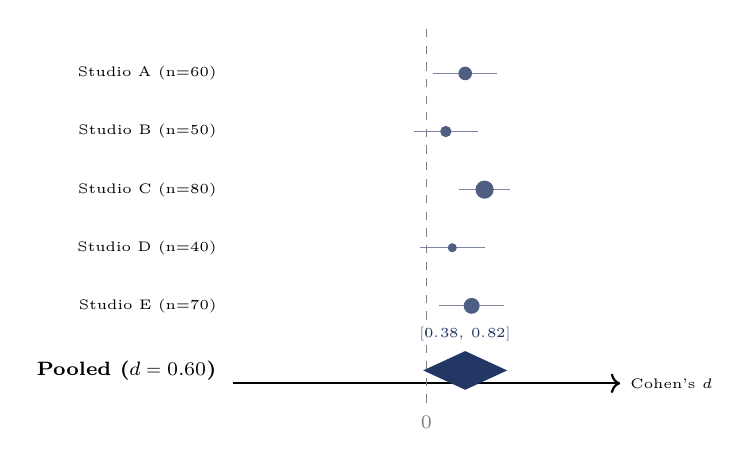
\begin{tikzpicture}[scale=0.82, font=\tiny]
  % Axes
  \draw[thick,->] (-3,0) -- (3,0) node[right]{Cohen's $d$};
  \draw[dashed,gray] (0,-0.3)--(0,5.5);
  \node[below,font=\scriptsize,gray] at (0,-0.35) {0};

  % Studies (point estimate + CI)
  \foreach \y/\est/\lo/\hi/\lbl/\w in {
    4.8 / 0.6 / 0.1 / 1.1 / {Studio A (n=60)}  / 3pt,
    3.9 / 0.3 /-0.2 / 0.8 / {Studio B (n=50)}  / 2.5pt,
    3.0 / 0.9 / 0.5 / 1.3 / {Studio C (n=80)}  / 4pt,
    2.1 / 0.4 /-0.1 / 0.9 / {Studio D (n=40)}  / 2pt,
    1.2 / 0.7 / 0.2 / 1.2 / {Studio E (n=70)}  / 3.5pt
  }{
    \draw[mblue!60] (\lo,\y)--(\hi,\y);
    \fill[mblue!80] (\est,\y) circle (\w);
    \node[left,font=\tiny] at (-3.1,\y) {\lbl};
  }
  % Pooled (diamond)
  \fill[mblue] (-0.05,0.2) -- (0.6,0.5) -- (1.25,0.2) -- (0.6,-0.1) -- cycle;
  \node[left,font=\scriptsize\bfseries] at (-3.1,0.2) {Pooled ($d = 0.60$)};
  \node[above,font=\tiny,mblue] at (0.6,0.5) {$[0.38,\; 0.82]$};
\end{tikzpicture}
\end{center}
\vspace{-0.3em}
\small Il \textbf{Forest Plot} mostra l'effect size e il suo IC 95\% per ogni studio. Il \textbf{diamante} rappresenta la stima pooled. Cerchi più grandi = studi con peso maggiore (n maggiore).
\end{frame}

\begin{frame}{Funnel Plot e Publication Bias}
\phantomsection\label{funnel-plot-e-publication-bias}
\begin{center}
\includegraphics[width=0.8\linewidth,height=\textheight,keepaspectratio]{Figures/Funnel_plot.png}
\end{center}

\small Un \textbf{funnel plot simmetrico} indica assenza di publication bias. L'\textbf{asimmetria} (lato sinistro vuoto) suggerisce che studi piccoli con effetti negativi non sono stati pubblicati.
\end{frame}

\begin{frame}{Eterogeneità: \(I^2\) e \(Q\) di Cochran}
\phantomsection\label{eterogeneituxe0-i2-e-q-di-cochran}
\small

\textbf{\(Q\) di Cochran}: testa se la variabilità tra studi è maggiore
di quella attesa per puro caso. Poco potente con pochi studi.

\vspace{0.3em}

\textbf{\(I^2\)} (Higgins): percentuale della variabilità totale
attribuibile all'eterogeneità vera (non campionaria).

\vspace{0.3em}

\begin{longtable}[]{@{}ll@{}}
\toprule\noalign{}
\(I^2\) & Interpretazione convenzionale \\
\midrule\noalign{}
\endhead
\footnotesize 0--25\% & \footnotesize Eterogeneità bassa \\
\footnotesize 25--50\% & \footnotesize Eterogeneità moderata \\
\footnotesize 50--75\% & \footnotesize Eterogeneità sostanziale \\
\footnotesize \(>75\%\) & \footnotesize Eterogeneità considerevole \\
\bottomrule\noalign{}
\end{longtable}

\vspace{0.3em}

\small \textbf{Attenzione}: alta eterogeneità non significa che la
meta-analisi sia sbagliata, ma che la stima pooled va interpretata con
cautela. Potrebbe essere necessaria un'analisi per \textbf{sottogruppi}
o una \textbf{meta-regressione}.
\end{frame}

\begin{frame}{Eterogeneità: approfondimenti}
\phantomsection\label{eterogeneituxe0-approfondimenti}
Per un approfondimento si veda
\href{https://pmc.ncbi.nlm.nih.gov/articles/PMC12326561/}{\underline{\textbf{Choi et al., 2025}}}
\end{frame}

\begin{frame}{Valutare il Publication Bias}
\phantomsection\label{valutare-il-publication-bias}
\small

\textbf{Funnel plot} (visivo): soggettivo; affidabile solo con
\(\geq 10\) studi.

\vspace{0.3em}

\textbf{Test di Egger}: regressione dell'effect size sulla sua
precisione: intercetta \(\neq 0\) suggerisce asimmetria.

\vspace{0.3em}

\textbf{Trim-and-Fill} (Duval \& Tweedie): stima quanti studi
``mancanti'' ci sarebbero in uno scenario simmetrico e corregge la stima
pooled.

\vspace{0.3em}

\textbf{\(p\)-curve e \(z\)-curve}: analizzano la distribuzione dei
\(p\)-value: possono rilevare \(p\)-hacking e selective reporting anche
senza funnel plot.

\vspace{0.3em}

\textbf{Fail-safe N} (Rosenthal): quanti studi negativi sarebbero
necessari per annullare il risultato? Meno usato oggi.

\vspace{0.2em}

\tiny Carter et al.~(2019). Correcting for bias in psychology: A
comparison of meta-analytic methods.
\emph{Advances in Methods and Practices in Psychological Science}. Open
Access: \url{https://journals.sagepub.com/doi/10.1177/2515245919847196}
\end{frame}

\begin{frame}{Risk of Bias (RoB)}
\phantomsection\label{risk-of-bias-rob}
\small

Ogni studio incluso nella meta-analisi viene valutato per il suo
\textbf{rischio di bias}, che influenza il peso che gli viene attribuito
e la fiducia nelle conclusioni.

\vspace{0.4em}

\textbf{Strumenti principali}:

\begin{itemize}\footnotesize
\item \textbf{RoB 2} (Cochrane, per RCT): 5 domini — randomizzazione, deviazioni dall'intervento, dati mancanti, misura dell'outcome, selezione dei risultati
\item \textbf{ROBINS-I} (per studi osservazionali): 7 domini
\item \textbf{QUADAS-2} (per studi diagnostici): 4 domini
\item \textbf{Newcastle-Ottawa Scale}: per studi di coorte e caso-controllo
\end{itemize}

\vspace{0.4em}

\textbf{Come si usa il RoB nella meta-analisi}: analisi di sensitività
escludendo gli studi ad alto rischio; ``GRADE'' per il livello
complessivo di evidenza.

\vspace{0.2em}

\tiny Sterne et al.~(2019). RoB 2: a revised tool for RCTs. \emph{BMJ}
366:l4898. Open Access: \url{https://doi.org/10.1136/bmj.l4898}
\end{frame}

\begin{frame}{Limiti Principali delle Meta-analisi}
\phantomsection\label{limiti-principali-delle-meta-analisi}


\begin{center}
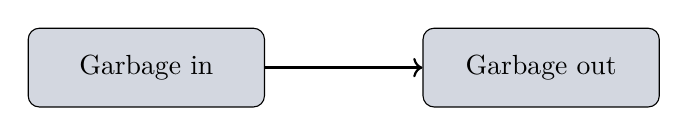
\begin{tikzpicture}[
  box/.style={draw, rounded corners, minimum width=3cm, minimum height=1cm, align=center, fill=mblue!20,}
]
  \node[box] (Gin) {Garbage in};
  \node[box, right=2cm of Gin] (Gout) {Garbage out};
  \draw[->, thick] (Gin) -- (Gout);
\end{tikzpicture}
\end{center}
\end{frame}

\begin{frame}{Limiti delle Meta-analisi}
\phantomsection\label{limiti-delle-meta-analisi}
\small

\textbf{``Garbage in, garbage out''}: se gli studi primari hanno bias
metodologici gravi, la meta-analisi li amplifica, non li corregge.

\vspace{0.3em}

\textbf{Publication bias}: gli studi con risultati significativi sono
più facilmente pubblicati \(\Rightarrow\) la letteratura disponibile è
distorta.

\vspace{0.3em}

\textbf{Eterogeneità eccessiva}: studi troppo diversi per popolazioni,
misure, interventi --- la stima pooled può essere priva di senso clinico
(``apples and oranges'').

\vspace{0.3em}

\textbf{Duplicazione di dati}: studi multipli sullo stesso dataset non
sono indipendenti.

\vspace{0.3em}

\textbf{Outcome switching}: gli studi primari riportano selettivamente
gli outcome significativi.

\vspace{0.3em}

\textbf{Aggregation bias (ecological fallacy)}: effetti a livello di
gruppo non necessariamente si applicano all'individuo.
\end{frame}

\begin{frame}{Psicometria e meta-analisi}
\phantomsection\label{psicometria-e-meta-analisi}
Esistono numerosi approcci che hanno come scopo incorporare elementi di
\textbf{psicometria} (es. affidabilità) nei risultati delle meta
analisi.

Questo puà avvenire ``analiticamente'' o tramite checklist di RoB.

Esempi di metodi analitici:

\begin{itemize}
\item
  Hunter \& Schmidt (2015) \emph{Methods of Meta-Analysis: Correcting
  Error and Bias in Research Findings.}
\item
  Jak \& Cheung (2020)
  \href{https://files.osf.io/v1/resources/ce85j/providers/osfstorage/5bf7eb3ec21cd8001aa31ac9?action=download&version=4&direct}{\underline{\textbf{Download Article}}}
\end{itemize}

Esempi di Checklist

\begin{itemize}
\tightlist
\item
  Mokking et al.~(2024). The COSMIN 2.0 checklist \ldots{} \emph{Quality
  of Life Research.}
  \href{https://pmc.ncbi.nlm.nih.gov/articles/PMC11541334/pdf/11136_2024_Article_3761.pdf}{\underline{\textbf{Download Article}}}
\end{itemize}
\end{frame}

\begin{frame}{Problemi Sistemici nelle Evidenze Cliniche}
\phantomsection\label{problemi-sistemici-nelle-evidenze-cliniche}
\small

\textbf{Small N e underpowered studies}

La maggioranza degli studi in neuropsicologia ha campioni insufficienti
per rilevare effetti piccoli. Con campioni piccoli, se l'effetto è
significativo, tende a essere sovrastimato (\textbf{Winner's curse}).

\vspace{0.4em}

\textbf{Questionable Research Practices (QRPs)}

\begin{itemize}\footnotesize
\item \emph{$p$-hacking}: testare più analisi finché $p < 0.05$
\item \emph{HARKing}: Hypothesizing After Results are Known — presentare come ipotesi ciò che è emerso dai dati
\item \emph{Outcome switching}: cambiare l'outcome primario dopo aver visto i dati
\end{itemize}

\vspace{0.4em}
\end{frame}

\section{12.4 Linee Guida e Consenso}\label{linee-guida-e-consenso}

\begin{frame}{Linee Guida Cliniche}
\phantomsection\label{linee-guida-cliniche}
\small

Le \textbf{linee guida} traducono le evidenze scientifiche in
raccomandazioni per la pratica clinica.

\vspace{0.4em}

\textbf{Come si costruiscono}:

\begin{enumerate}\footnotesize
\item Panel multidisciplinare di esperti
\item Revisione sistematica delle evidenze disponibili
\item Valutazione della qualità delle evidenze con sistema \textbf{GRADE}
\item Formulazione delle raccomandazioni (forza e direzione)
\item Revisione esterna e aggiornamento periodico
\end{enumerate}

\vspace{0.4em}
\end{frame}

\begin{frame}{Il sistema GRADE}
\phantomsection\label{il-sistema-grade}
\textbf{Sistema GRADE} (Grading of Recommendations Assessment,
Development and Evaluation):

\begin{itemize}\footnotesize
\item Qualità evidenze: Alta / Moderata / Bassa / Molto Bassa
\item Forza raccomandazione: Forte / Debole (condizionale)
\end{itemize}

\vspace{0.2em}

\tiny Guyatt et al.~(2008). GRADE: An emerging consensus. \emph{BMJ}
336:924. Open Access: \url{https://doi.org/10.1136/bmj.39489.470347.AD}
\end{frame}

\begin{frame}{Delphi Consensus}
\phantomsection\label{delphi-consensus}
\small

Quando le evidenze sono scarse o insufficienti per linee guida basate su
sistematiche, si ricorre al \textbf{metodo Delphi} per sintetizzare
l'\textbf{opinione di esperti} in modo strutturato.

\vspace{0.4em}

\textbf{Procedura}:

\begin{enumerate}\footnotesize
\item Selezione di un panel di esperti (anonimato garantito)
\item Round 1: questionario aperto — gli esperti esprimono opinioni
\item Sintesi delle risposte e feedback al panel
\item Round 2 (e seguenti): gli esperti rivalutano le proprie posizioni alla luce del gruppo
\item Il processo si ripete fino al raggiungimento del \textbf{consenso} (es.\ $\geq 70\%$ accordo)
\end{enumerate}

\vspace{0.4em}
\end{frame}

\begin{frame}{Delphi in neuropsicologia o psicologia}
\phantomsection\label{delphi-in-neuropsicologia-o-psicologia}
\textbf{Uso in neuropsicologia}: definizione di criteri diagnostici
(es.~MCI), raccomandazioni per la valutazione neuropsicologica in
condizioni rare, standard di pratica in assenza di RCT.

\vspace{0.2em}

\tiny Fink (2019). \emph{The Delphi Method: Technique and Applications}.
\end{frame}

\begin{frame}{GRADE e Forza delle Raccomandazioni}
\phantomsection\label{grade-e-forza-delle-raccomandazioni}
\begin{center}
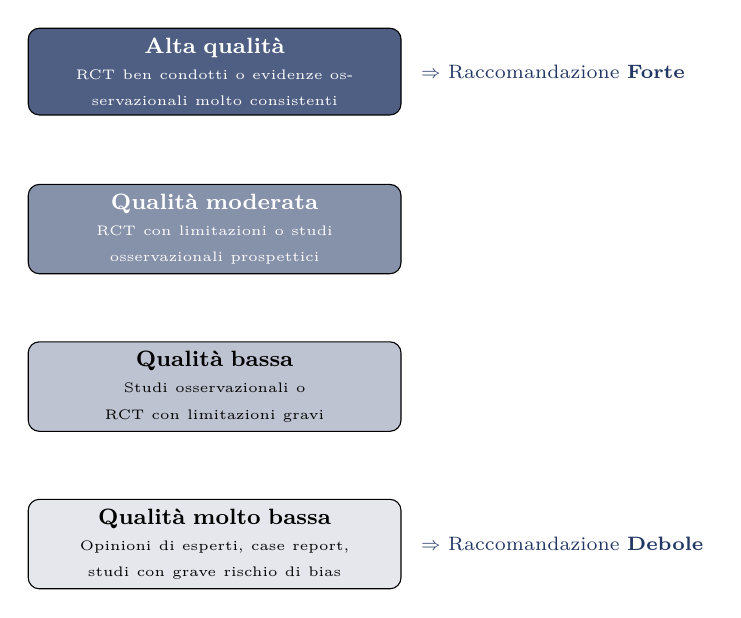
\begin{tikzpicture}[
  box/.style={draw, rounded corners, text width=4.5cm, align=center,
              font=\footnotesize, minimum height=0.9cm},
]
\node[box, fill=mblue!80, text=white] at (0,4)
  {\textbf{Alta qualità}\\\tiny RCT ben condotti o evidenze osservazionali molto consistenti};
\node[box, fill=mblue!55, text=white] at (0,2)
  {\textbf{Qualità moderata}\\\tiny RCT con limitazioni o studi osservazionali prospettici};
\node[box, fill=mblue!30] at (0,0)
  {\textbf{Qualità bassa}\\\tiny Studi osservazionali o RCT con limitazioni gravi};
\node[box, fill=mblue!12] at (0,-2)
  {\textbf{Qualità molto bassa}\\\tiny Opinioni di esperti, case report, studi con grave rischio di bias};
\node[right, font=\scriptsize, mblue] at (2.5,4) {$\Rightarrow$ Raccomandazione \textbf{Forte}};
\node[right, font=\scriptsize, mblue] at (2.5,-2) {$\Rightarrow$ Raccomandazione \textbf{Debole}};
\end{tikzpicture}
\end{center}
\end{frame}

\begin{frame}{Riepilogo: Dal Singolo Studio alla Pratica}
\phantomsection\label{riepilogo-dal-singolo-studio-alla-pratica}
\begin{center}
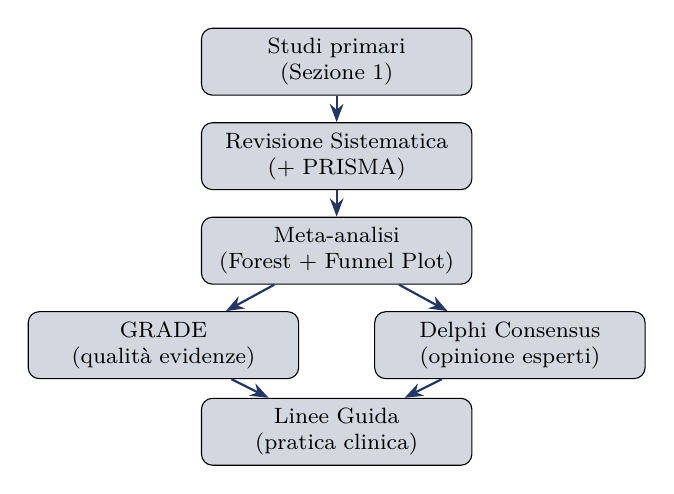
\begin{tikzpicture}[
  box/.style={draw, rounded corners, fill=mblue!20, text width=3.2cm,
              align=center, font=\footnotesize, minimum height=0.85cm},
  arr/.style={-{Stealth}, mblue, thick}
]
\node[box] (st) at (0,4.5)  {Studi primari\\(Sezione 1)};
\node[box] (sr) at (0,3.3)  {Revisione Sistematica\\(+ PRISMA)};
\node[box] (ma) at (0,2.1)  {Meta-analisi\\(Forest + Funnel Plot)};
\node[box] (gr) at (-2.2,0.9){GRADE\\(qualità evidenze)};
\node[box] (dp) at ( 2.2,0.9){Delphi Consensus\\(opinione esperti)};
\node[box] (lg) at (0,-0.2) {Linee Guida\\(pratica clinica)};
\draw[arr] (st)--(sr); \draw[arr] (sr)--(ma);
\draw[arr] (ma)--(gr); \draw[arr] (ma)--(dp);
\draw[arr] (gr)--(lg); \draw[arr] (dp)--(lg);
\end{tikzpicture}
\end{center}
\end{frame}




\end{document}
